\title{Introductory Electricity, Magnetism, and Optics Practice Problems}
\author{Cyrus Vandrevala}

\documentclass[11pt]{article}
\usepackage[margin=2.5cm]{geometry}
\usepackage[pdftex]{graphicx}

\begin{document}

\maketitle
\tableofcontents
\vspace{50pt}

\subsection*{Useful Constants}
Electron Mass = $9.11 \times 10^{-31}$ kg \\*
Proton Mass = $1.67 \times 10^{-27}$ kg \\*
Elementary Charge = $1.602 \times 10^{-19}$ C \\*
Coulomb's Constant = $8.99 \times 10^9$ Nm$^2$/C$^2$ \\*
Gravitational Constant = $6.67 \times 10^{-11}$ m$^3$/kg$\cdot s^2$
Avogadro's Number = $ 6.02 \times 10^{23}$ atoms/mole \\*\\*
Atomic Number of Uranium = 92 \\*
Atomic Number of Copper = 29 \\*
Molar Mass of Copper = 63.5 g/mole \\*
Mass of the Earth = $5.97 \times 10^{24}$ kg\\*
Mass of the Moon = $7.35 \times 10^{22}$ kg

%%%%%%%%%%%%%%%%%%%%%%%%%%%%%%%%%%%%%%%%%%%%%%%%%%%%%%%%%%%%%%%%%%%%%%%%%%%%%%%%%%%%%%%%%%%%

\pagebreak
\section{Quantized Electric Charge and Charging Objects}
\vspace{10pt}

\subsection{Transfer of Electrons}
I rub a piece of silk against a glass rod in order to charge up the rod.  If the final charge on the rod is +2.3 $\mu$C, how many electrons were transferred from the rod to the silk?

\subsection{Charge Within a Uranium Nucleus}
What is the net charge within the nucleus of an atom of U-238?

\subsection{Number of Electrons in Copper}
Estimate the number of electrons in a 1.0 kg block of copper that has been charged to +10 $\mu$C.

\subsection{Charging an Object \#1}
I bring a charged insulator close to an uncharged conductor (not touching).  I then ground the conductor.  This method of charging the conductor is called charging by \underline{\hspace{1cm}}.

\subsection{Charging an Object \#2}
I touch an uncharged conductor to a second negatively charged conductor.  This method of charging an object is called charging by \underline{\hspace{1cm}}.

\subsection{Charging an Object \#3}
I rub a glass rod against a silk cloth in order to charge up the glass rod.  This is an example of charging by \underline{\hspace{1cm}}.

%%%%%%%%%%%%%%%%%%%%%%%%%%%%%%%%%%%%%%%%%%%%%%%%%%%%%%%%%%%%%%%%%%%%%%%%%%%%%%%%%%%%%%%%%%%%

\pagebreak
\section{Coulomb's Force Law}
\vspace{10pt}

\subsection{Hydrogen Atom}
In a hydrogen atom, a proton is separated from an electron by an average distance of about $5.3 \times 10^{-11}$ meters.  Calculate the electrostatic force of attraction by the proton on the electron.  Do the same for the electron on the proton.

\subsection{Force at the Center of a Square}
Suppose I place four charges (each +Q) at the four vertices of a square with side length L.  What is the magnitude of the net force on a positive point charge (+q) located at the center of the square?

\subsection{Equilibrium Point}
Suppose I place a charge of $Q_1$ = +1.0 nC at the point (1 m, 0 m) and a charge of $Q_2$ = -2.5 nC at the point (0 m, 0 m).  At what point in the xy-plane could I put a negative charge of $Q_3$ = -5.0 $\mu$C such that $Q_3$ would feel no net electrostatic force?

\subsection{Electrical vs. Gravitational Force}
Suppose the moon were held in orbit due to an electrical force instead of a gravitational force.  Assume that the Earth and the moon have equal charge magnitudes with opposite sign (i.e. $Q_{Earth}$ = +q and $Q_{Moon}$ = -q).  How large would these charges have to be in order to maintain the current stable orbit?

\subsection{Charged Pendulum}
Consider the double pendulum setup shown below.  Two small spherical bobs, each with mass M and charge Q hang from strings of length L.  After a short time, the bobs reach the equilibrium position as shown.  Calculate an expression for the angle $\theta$ when the bobs come to equilibrium.\\*

\begin{center}
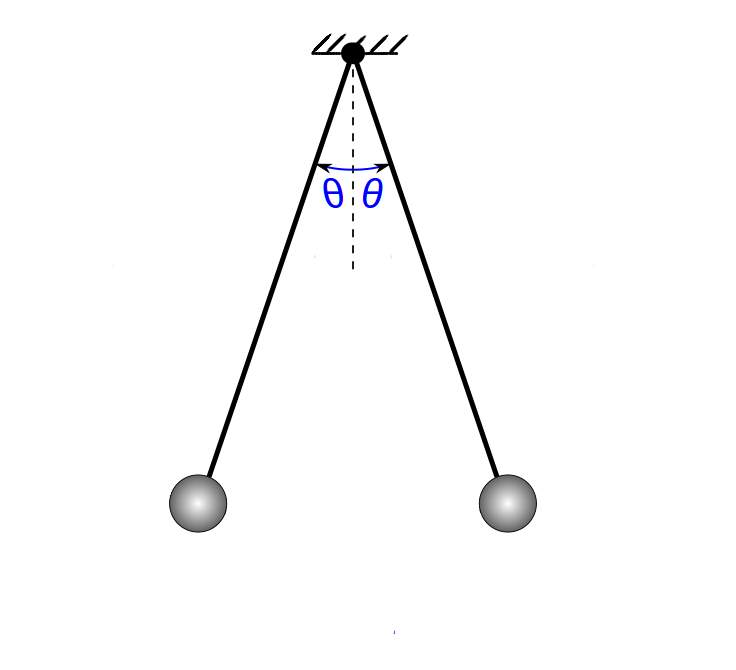
\includegraphics[scale=0.25]{Images/pendulum.png}
\end{center}

%%%%%%%%%%%%%%%%%%%%%%%%%%%%%%%%%%%%%%%%%%%%%%%%%%%%%%%%%%%%%%%%%%%%%%%%%%%%%%%%%%%%%%%%%%%%

\pagebreak
\section{Continuous Electric Charge}
\vspace{10pt}

\subsection{Charge at the Center of a Ring}
Consider a charged ring in the xy-plane, centered at the origin, with charge density $\rho$ = cos($\theta$) where $\theta$ is the angle about the ring in standard orientation.  If I place a positive charge at the center of the ring, which way will it move?

\subsection{Uniformly Charged Ring}
Calculate the electric field along the axis of a uniformly charged ring (radius R, net charge Q).

\subsection{Uniformly Charged Ring (Difficult - Extra Credit)}
Show that for small distances, the electric field around the center of the uniformly charged ring is linear with distance.  Then, show that a particle released near the center of the ring experiences simple harmonic motion.

\subsection{Charged Line \#1}
A uniform line of charge extends from the point (0,0) to (1,0).  It has a net charge of +Q.  What is the electric field at the point (2,0)?

\subsection{Charged Line \#2}
A uniform line of charge extends from the point (0,0) to (1,0).  It has a net charge of +Q.  What is the electric field at the point (2,1)?

%%%%%%%%%%%%%%%%%%%%%%%%%%%%%%%%%%%%%%%%%%%%%%%%%%%%%%%%%%%%%%%%%%%%%%%%%%%%%%%%%%%%%%%%%%%%

\pagebreak
\section{Electric Field}
\vspace{10pt}

\subsection{Electron in an Electric Field \#1}
An electron is fired into a uniform electric field.  The initial velocity of the electron is given by $\vec{v} = 500 \hat{x} + 100 \hat{y} - 300 \hat{z}$, and the electric field is given by $\vec{E} = 100 \hat{x} + 200 \hat{y} - 150 \hat{z}$.  Calculate the acceleration of the electron.

\subsection{Electron in an Electric Field \#2}
An electron is fired into a region of uniform electric field given by $\vec{E} = 100\hat{y}$. At time t = 0 s, it is located at the origin with an initial velocity of $\vec{v_o} = 5.0 \times 10^5 \hat{x} + 3 \times 10^5 \hat{y}$  m/s.  What is the velocity of the particle at time t = 10 s?

\subsection{Electron in an Electric Field \#3}
An electron is fired into a region of uniform electric field given by $\vec{E} = 100\hat{y}$. At time t = 0 s, it is located at the origin with an initial velocity of $\vec{v_o} = 5.0 \times 10^5 \hat{x} + 3 \times 10^5 \hat{y}$ m/s.  At what time during its trajectory does it intersect the x-axis again?

\subsection{Multiple Choice}
Which of the following statements is NOT true?

\begin{itemize}
	\item[A)] Electric field lines emanate from positive charges and terminate on negative charges.
	\item[B)] Electric field lines that are closely spaced imply a strong electric field.
	\item[C)] Positive point charges feel an electric force parallel to electric field lines.
	\item[D)] A positive point charge does NOT produce an electric field.
\end{itemize}

\subsection{Pendulum in an Electric Field}
Consider a simple pendulum that has a bob with mass M and charge +Q as shown below.  The string of the pendulum has a length L.  A uniform electric field of magnitude E keeps the pendulum bob at equilibrium.  Derive an expression for $\theta$.\\*

\begin{center}
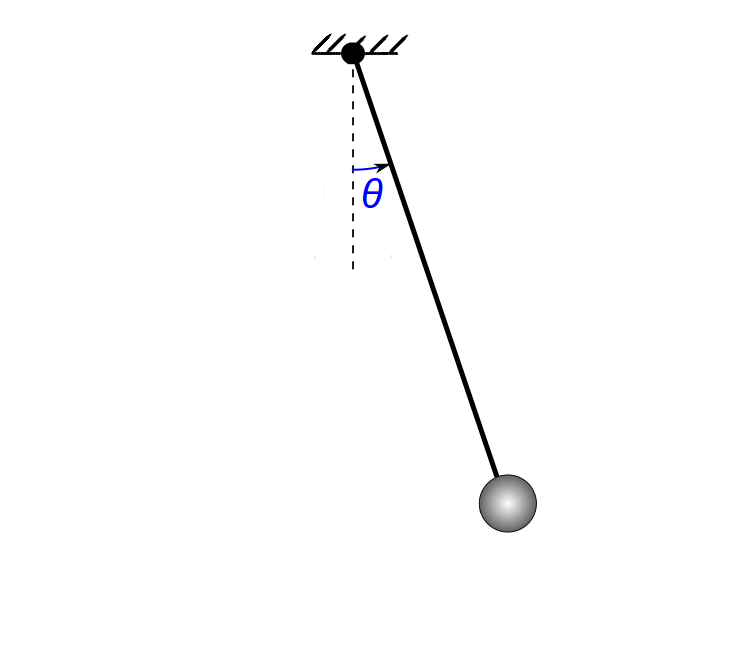
\includegraphics[scale=0.25]{Images/pendulum-efield.png}
\end{center}
%%%%%%%%%%%%%%%%%%%%%%%%%%%%%%%%%%%%%%%%%%%%%%%%%%%%%%%%%%%%%%%%%%%%%%%%%%%%%%%%%%%%%%%%%%%%

\pagebreak
\section{Electric Dipoles}
\vspace{10pt}

\subsection{Electric Field Due to a Dipole}
Consider an electric dipole with charges +Q and -Q located at x = +1 m and x = -1 m respectively.  Calculate the net electric field due to the dipole at x = 0 m.

\subsection{Potential Energy of an Electric Dipole}
I place a dipole with dipole moment p = 10$\hat{z}$ C$\cdot$m in an electric field E = -100$\hat{x}$ N/C.  What is the potential energy of the dipole?

\subsection{Maximum Potential Energy of an Electric Dipole}
Suppose I put a polar object with dipole moment 2.00 C$\cdot$m in a uniform electric field of magnitude 300 N/C.  What is the maximum possible value for the potential energy of the system?

\subsection{Multiple Choice}
Which of the following statements is NOT true?

\begin{itemize}
	\item[A)] If a perfect electric dipole is placed into a uniform electric field, it can experience a net force.
	\item[B)] A perfect electric dipole consists of two equal and opposite point charges separated by a small distance.
	\item[C)] If a perfect electric dipole is placed into a non-uniform electric field, the dipole can experience a net force.
	\item[D)] If a perfect electric dipole is placed into a uniform electric field, the dipole can experience a net torque.
	\item[E)] If a perfect electric dipole is placed into a non-uniform electric field, the dipole can experience a net force.
\end{itemize}

%%%%%%%%%%%%%%%%%%%%%%%%%%%%%%%%%%%%%%%%%%%%%%%%%%%%%%%%%%%%%%%%%%%%%%%%%%%%%%%%%%%%%%%%%%%%

\pagebreak
\section{Electric Flux}

\subsection{Charge Density}
Charge per unit volume is defined as \underline{\hspace{1cm}}.

\subsection{Flux Through a Sphere}
Some region of space contains a uniform electric field given by $\vec{E} = 3\hat{i} + 4\hat{j}$ N/C.  I place a metal spherical shell of radius R = 1 m into the electric field.  What is the net electric flux through the sphere?

\subsection{Flux Around an Electric Dipole}
An electric dipole is formed by two point charges - +Q and -Q located (1 m, 0 m) and (-1 m, 0 m) respectively.  I draw a closed elliptical surface such that the charges +Q and -Q are both outWhat is the net electric flux through the green ellipse?

%%%%%%%%%%%%%%%%%%%%%%%%%%%%%%%%%%%%%%%%%%%%%%%%%%%%%%%%%%%%%%%%%%%%%%%%%%%%%%%%%%%%%%%%%%%%

\pagebreak
\section{Answers}
\vspace{15pt}

\subsection*{Quantized Electric Charge and Charging Objects}
\vspace{5pt}
\paragraph{1.1: Transfer of Electrons $\rightarrow$} 1.4 $\times$ 10$^{13}$ electrons
\paragraph{1.2: Charge Within a Uranium Nucleus $\rightarrow$} 1.5 $\times$ 10$^{-17}$ C
\paragraph{1.3: Number of Electrons in Copper $\rightarrow$} $2.7 \times 10^{26}$ electrons
\paragraph{1.4: Charging an Object \#1 $\rightarrow$} Induction
\paragraph{1.5: Charging an Object \#2 $\rightarrow$} Contact
\paragraph{1.6: Charging an Object \#3 $\rightarrow$} Friction
\vspace{15pt}

\subsection*{Coulomb's Force Law}
\paragraph{2.1: Hydrogen Atom $\rightarrow$} $8.2 \times 10^{-8}$ N, Same For Both
\paragraph{2.2: Force at the Center of a Square $\rightarrow$} 0 N
\paragraph{2.3: Equilibrium Point $\rightarrow$} (2.7 m, 0 m)
\paragraph{2.4: Electrical vs. Gravitational Force $\rightarrow$} $|Q_{Earth}| = |Q_{Moon}| = 5.71\times10^{13}$ C
\paragraph{2.5: Charged Pendulum $\rightarrow$} $\theta =$ arctan$(\frac{kQ^2}{mgd^2})$
\vspace{15pt}

\subsection*{Continuous Electric Charge}
\paragraph{3.1: Charge at the Center of a Ring $\rightarrow$} $-\hat{x}$ direction
\paragraph{3.2: Uniformly Charged Ring $\rightarrow$} $\vec{E} = \frac{kQz}{(z^2 + R^2)^{3/2}}\hat{z}$
\paragraph{3.3: Uniformly Charged Ring (Difficult - Extra Credit) $\rightarrow$} 
\begin{equation}
\vec{E} \approx \frac{kQz}{R^3} \rightarrow \vec{F} = m \vec{a}
\end{equation}
\begin{equation}
\Rightarrow -\frac{kQz}{R^3} = m\frac{d^2z}{dt^2} 
\end{equation}
\begin{equation}
\Rightarrow \frac{d^2z}{dt^2} + \frac{kQz}{mR^3} = 0 
\end{equation}
\begin{equation}
\Rightarrow z(t) = Asin(\omega t), \omega = \sqrt{\frac{kQ}{mR^3}}
\end{equation}
\paragraph{4.4 $\rightarrow$}
\paragraph{4.5 $\rightarrow$}

\subsection*{Electric Field}
\paragraph{5.1 $\rightarrow$} $\vec{a} = 4.735 \times 10^{13}$ m/s$^2$
\paragraph{5.2 $\rightarrow$}
\paragraph{5.3 $\rightarrow$}
\paragraph{5.4 $\rightarrow$} D

\subsection*{Electric Dipoles}
\paragraph{5.1: Electric Field Due to a Dipole $\rightarrow$} $-2kQ \hat{x}$
\paragraph{5.2: Potential Energy of an Electric Dipole $\rightarrow$} 0 J
\paragraph{5.3: Maximum Potential Energy of an Electric Dipole $\rightarrow$} 600 Nm
\paragraph{5.4: Multiple Choice $\rightarrow$} A

\subsection*{Electric Flux}

%%%%%%%%%%%%%%%%%%%%%%%%%%%%%%%%%%%%%%%%%%%%%%%%%%%%%%%%%%%%%%%%%%%%%%%%%%%%%%%%%%%%%%%%%%%%

\end{document}




